\documentclass[aspectratio=169,11pt]{beamer}
% Phase 1 presentation. Compile from this folder: pdflatex slides (run twice).
\usetheme{default}
\usecolortheme{dove}
\setbeamertemplate{navigation symbols}{}
\setbeamertemplate{footline}[frame number]
\usepackage{booktabs}
\usepackage{graphicx}
\graphicspath{{../results/figures/}}
\newcommand{\ugm}{$\mu$g/m$^3$}

\title{One-Hour-Ahead PM2.5 Forecasting in Beijing}
\subtitle{Gradient-boosted trees vs.\ naive baselines under a leakage-controlled protocol}
\author{Animesh Kumar Rai}
\date{Project 19 --- Phase 1}

\begin{document}

\begin{frame}
\titlepage
\end{frame}

\begin{frame}{Problem and question}
\begin{itemize}
\item Forecast PM2.5 at the US Embassy, Beijing, \textbf{one hour ahead}.
\item WHO 2021 24-hour guideline: 15 \ugm{}; Beijing often exceeds it by $10\times$.
\item At 1 h, PM2.5 barely changes, so ``next hour = this hour'' (persistence) is hard to beat.
\item \textbf{Question:} without leakage, how much does XGBoost beat naive baselines --- and where does it fail?
\end{itemize}
\end{frame}

\begin{frame}{Data: UCI Beijing PM2.5 (2010--2014)}
\begin{columns}
\column{0.48\textwidth}
\begin{itemize}
\item 43,824 hourly rows; complete hourly index.
\item PM2.5 missing 4.7\% (214 gaps, up to 155 h).
\item Weather from Capital Airport; wind is a \emph{cumulative} counter that we decode to hourly speed.
\item Skewed: median 72, max 994 \ugm{}.
\end{itemize}
\column{0.52\textwidth}
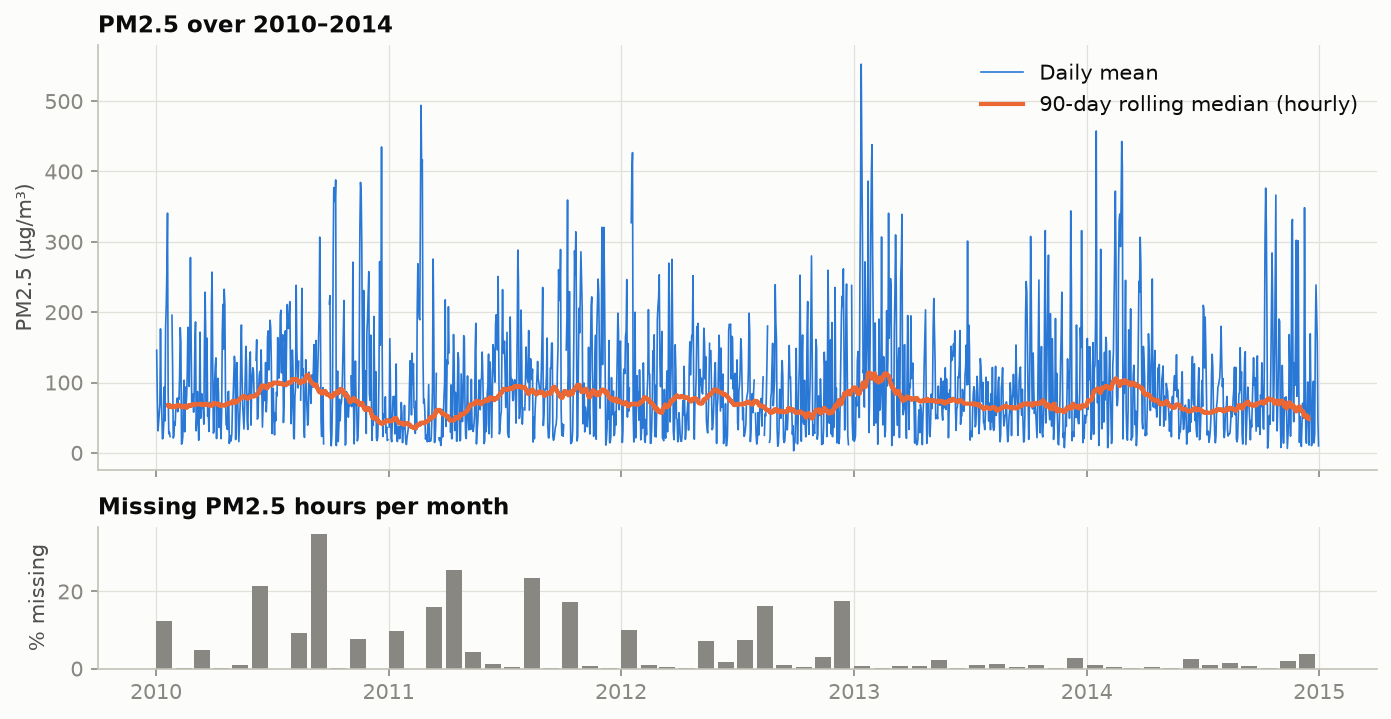
\includegraphics[width=\linewidth]{eda_02_timeseries_missingness.png}
\end{columns}
\end{frame}

\begin{frame}{What the EDA showed}
\begin{columns}
\column{0.5\textwidth}
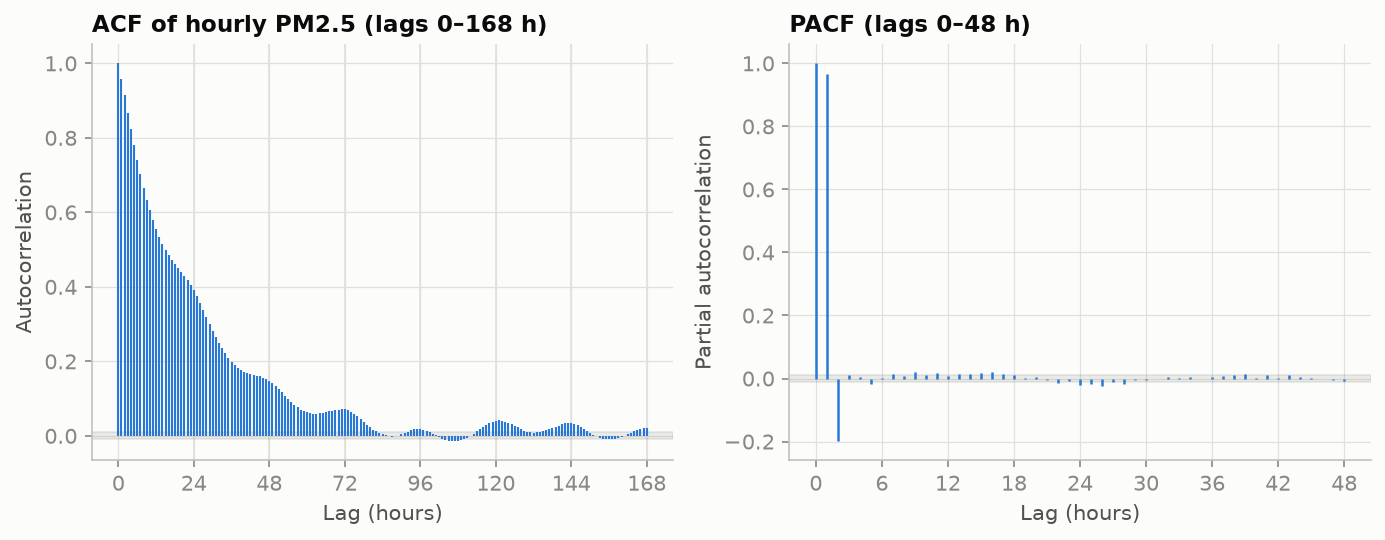
\includegraphics[width=\linewidth]{eda_06_acf_pacf.png}
\column{0.5\textwidth}
\begin{itemize}
\item ACF 0.96 at 1 h, 0.39 at 24 h, $\approx 0$ at 168 h.
\item PACF: lags 1--2 carry the direct information.
\item Daily cycle differs by season.
\item NW wind $\rightarrow$ clean air (median 31); calm $\rightarrow$ 98 \ugm{}.
\end{itemize}
\end{columns}
\end{frame}

\begin{frame}{Protocol: no peeking at the future}
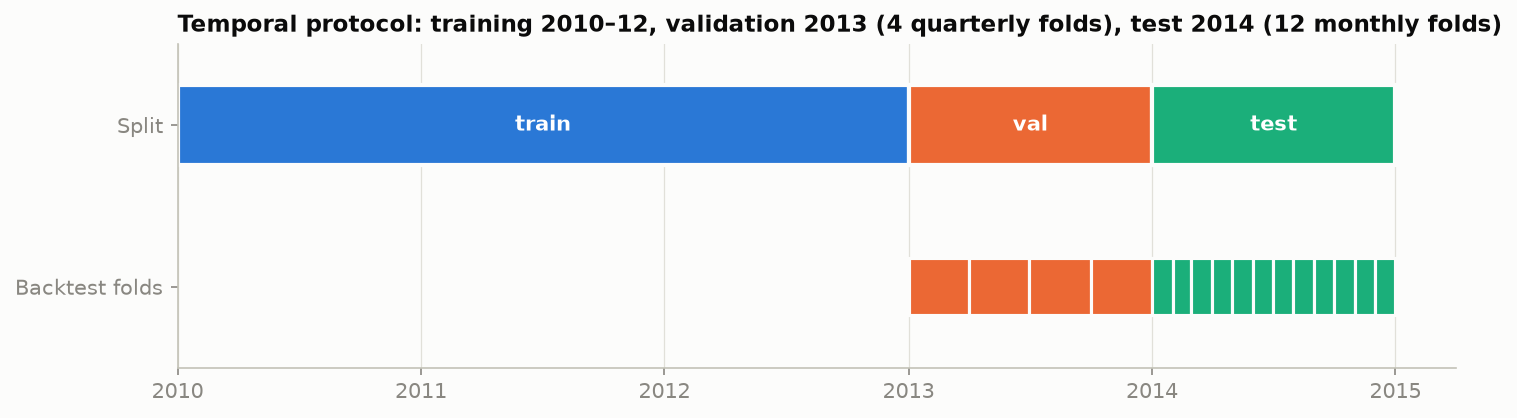
\includegraphics[width=\linewidth]{protocol_01_timeline.png}
\begin{itemize}
\item Issue at end of hour $t$; target $x_{t+1}$; inputs only from hours $\le t$.
\item Samples assigned by \textbf{target} time; whole-year splits.
\item Tune on 2013 quarters; test 2014 \textbf{once}, monthly refits, frozen settings.
\item Same scored hours for every model; no interpolation (it uses the future).
\end{itemize}
\end{frame}

\begin{frame}{Features (37, all past-only)}
\begin{itemize}
\item PM2.5 lags 0, 1, 2, 3, 6, 12, 23; last change; trailing mean/std (3--24 h).
\item Weather at $t$: dew point, temperature, pressure, spread, 3-h tendencies.
\item Wind: decoded hourly speed, direction persistence, one-hot direction.
\item Calendar of $t+1$: sin/cos hour and month, day of week.
\item \textbf{Leakage test:} randomise every row after $t$ $\Rightarrow$ features at $\le t$ unchanged (30 cut points).
\end{itemize}
\end{frame}

\begin{frame}{Baselines and a bit of theory}
\begin{itemize}
\item Persistence $\hat{y} = x_t$; seasonal-naive $\hat{y} = x_{t-23}$.
\item Naive lag-$k$: $\mathrm{MSE} = 2\sigma^2(1-\rho_k) \Rightarrow R^2 \approx 2\rho_k - 1$.
\item $\rho_{24} = 0.38 \Rightarrow R^2 \approx -0.23$ (observed $-0.22$): seasonal-naive is worse than the mean.
\item $\rho_1 = 0.95 \Rightarrow R^2 \approx 0.91$ (observed 0.92): persistence is the real bar.
\end{itemize}
\end{frame}

\begin{frame}{XGBoost: framing beats tuning}
\begin{columns}
\column{0.45\textwidth}
\begin{tabular}{lc}
\toprule
Target (2013 folds) & RMSE \\
\midrule
Level & 23.79 \\
log(1+level) & 24.31 \\
\textbf{Change} $x_{t+1}-x_t$ & \textbf{21.80} \\
Persistence & 23.70 \\
\bottomrule
\end{tabular}
\vspace{1em}

Tuned (40 configs): 21.41; seed std $\approx$ 0.04.
\column{0.55\textwidth}
\begin{itemize}
\item Trees are piecewise constant; copying $x_t$ costs many splits.
\item Learning only the \emph{change} removes that burden.
\end{itemize}
\end{columns}
\end{frame}

\begin{frame}{Test year 2014 (single evaluation)}
\begin{columns}
\column{0.42\textwidth}
\begin{tabular}{lcc}
\toprule
 & MAE & RMSE \\
\midrule
Persistence & 11.93 & 22.03 \\
Seasonal-naive & 67.30 & 98.75 \\
\textbf{XGBoost} & \textbf{10.96} & \textbf{19.96} \\
\bottomrule
\end{tabular}
\vspace{0.6em}
\begin{itemize}
\item $-8.1\%$ MAE, $-9.4\%$ RMSE; 12/12 months.
\item Diebold--Mariano $p < 10^{-6}$.
\end{itemize}
\column{0.58\textwidth}
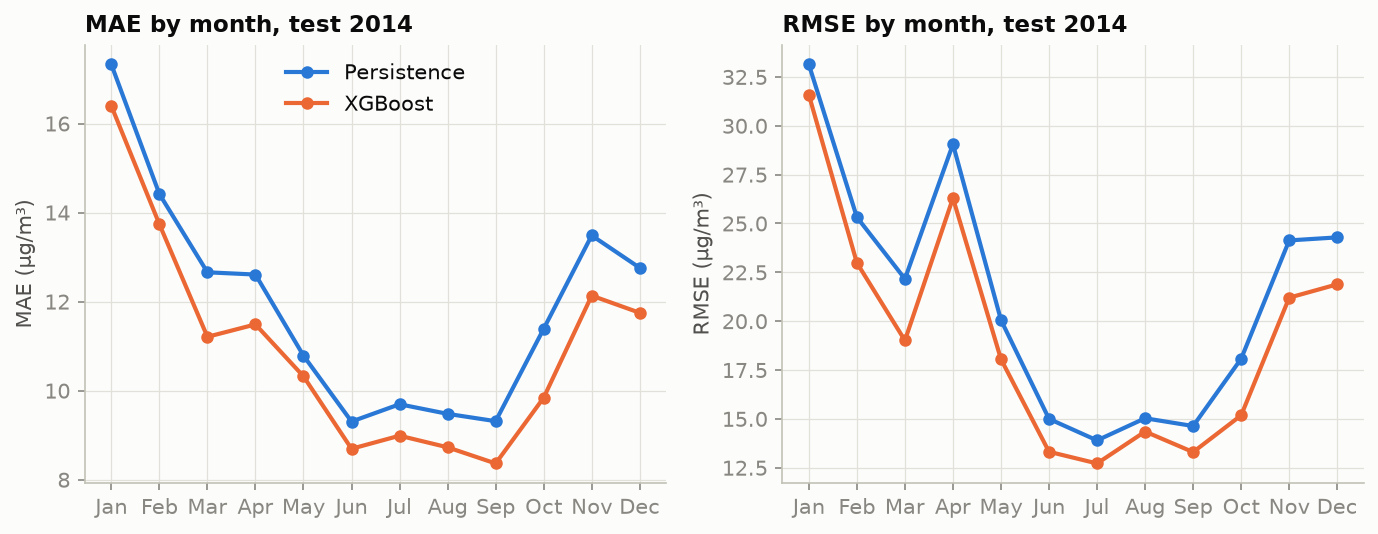
\includegraphics[width=\linewidth]{test_01_monthly.png}
\end{columns}
\end{frame}

\begin{frame}{Where it fails}
\begin{columns}
\column{0.5\textwidth}
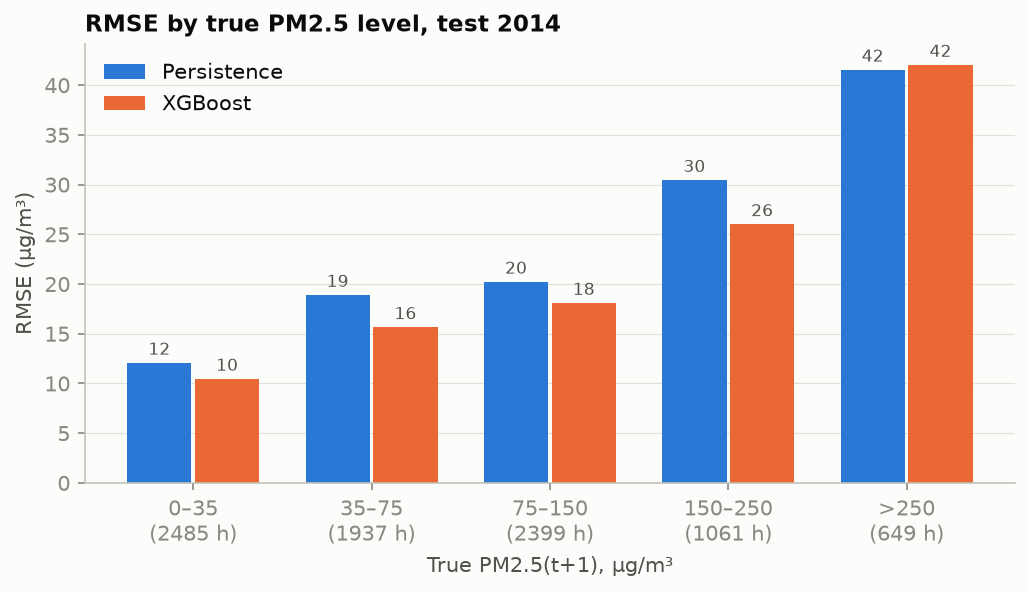
\includegraphics[width=\linewidth]{test_02_by_level.png}
\column{0.5\textwidth}
\begin{itemize}
\item $>250$ \ugm{}: no gain (RMSE 42.0 vs 41.6); under-predicts by 12.8.
\item Big falls: MAE 84.7 $\rightarrow$ 60.6 (NW wind onset visible in inputs).
\item Big rises: no gain (84.9 vs 85.1).
\item Stable hours: slightly worse (5.0 vs 4.0).
\end{itemize}
\end{columns}
\end{frame}

\begin{frame}{What drives the model}
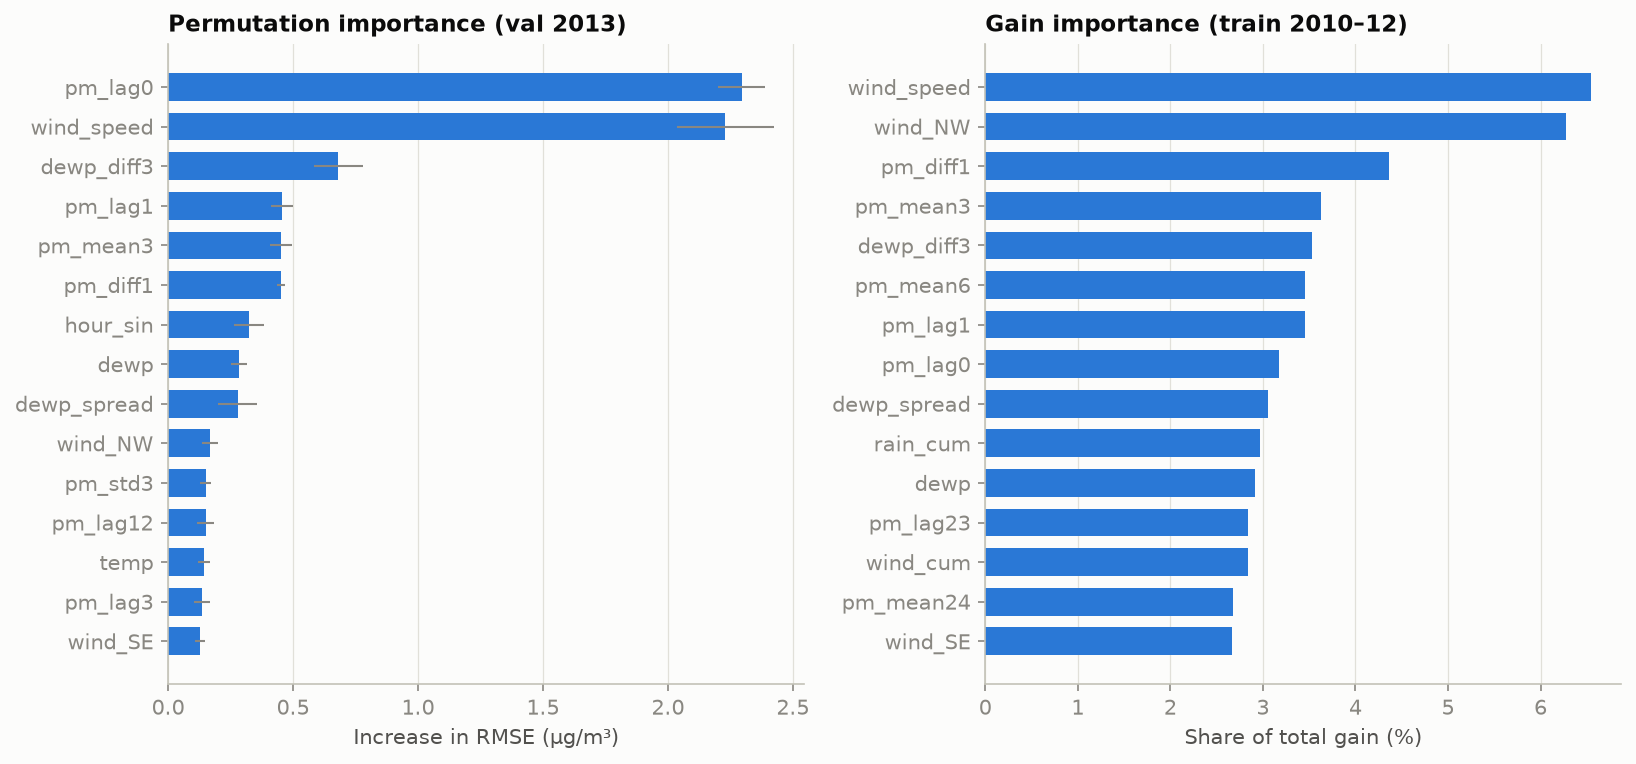
\includegraphics[width=\linewidth]{xgb_03_importance.png}
\small Current PM2.5 and decoded wind speed dominate. Importance shows association within the model, not causation.
\end{frame}

\begin{frame}{Conclusions and next steps}
\begin{itemize}
\item XGBoost beats persistence by $\approx 9\%$ RMSE --- real, consistent, significant, but modest.
\item Problem framing mattered more than hyperparameters.
\item Skill is asymmetric: anticipates clean-air arrival, not build-up or extremes.
\item Fully reproducible: a fresh environment regenerates all results byte for byte.
\item \textbf{Phase 2:} LSTM under the same protocol; tail-aware losses.
\item Limits: one station, one test year, observed (not forecast) weather.
\end{itemize}
\end{frame}

\end{document}
